% 波-粒(局部连接)二象性
% 波和连接同时考虑比单独一个精度更高
% 全局的波在局部形成共振

% Alex --> 神经场理论中的深度学习 -> 几何约束
% https://github.com/kwignb/RandomNeuralField/blob/main/src/models/networks.py

% 神经场介绍
%Version 3 October 2023
% See section 11 of the User Manual for version history
%
%%%%%%%%%%%%%%%%%%%%%%%%%%%%%%%%%%%%%%%%%%%%%%%%%%%%%%%%%%%%%%%%%%%%%%
%%                                                                 %%
%% Please do not use \input{...} to include other tex files.       %%
%% Submit your LaTeX manuscript as one .tex document.              %%
%%                                                                 %%
%% All additional figures and files should be attached             %%
%% separately and not embedded in the \TeX\ document itself.       %%
%%                                                                 %%
%%%%%%%%%%%%%%%%%%%%%%%%%%%%%%%%%%%%%%%%%%%%%%%%%%%%%%%%%%%%%%%%%%%%%

%%\documentclass[referee,sn-basic]{sn-jnl}% referee option is meant for double line spacing

%%=======================================================%%
%% to print line numbers in the margin use lineno option %%
%%=======================================================%%

%%\documentclass[lineno,sn-basic]{sn-jnl}% Basic Springer Nature Reference Style/Chemistry Reference Style

%%======================================================%%
%% to compile with pdflatex/xelatex use pdflatex option %%
%%======================================================%%

%%\documentclass[pdflatex,sn-basic]{sn-jnl}% Basic Springer Nature Reference Style/Chemistry Reference Style


%%Note: the following reference styles support Namedate and Numbered referencing. By default the style follows the most common style. To switch between the options you can add or remove “Numbered” in the optional parenthesis. 
%%The option is available for: sn-basic.bst, sn-vancouver.bst, sn-chicago.bst%  
 
%%\documentclass[sn-nature]{sn-jnl}% Style for submissions to Nature Portfolio journals
%%\documentclass[sn-basic]{sn-jnl}% Basic Springer Nature Reference Style/Chemistry Reference Style


% 需要将bst目录下的sn-mathphys-num.bst复制到根目录下,否则参考文献为问号
\documentclass[sn-mathphys-num]{sn-jnl}% Math and Physical Sciences Numbered Reference Style 
%%\documentclass[sn-mathphys-ay]{sn-jnl}% Math and Physical Sciences Author Year Reference Style
%%\documentclass[sn-aps]{sn-jnl}% American Physical Society (APS) Reference Style
%%\documentclass[sn-vancouver,Numbered]{sn-jnl}% Vancouver Reference Style
%%\documentclass[sn-apa]{sn-jnl}% APA Reference Style 
%%\documentclass[sn-chicago]{sn-jnl}% Chicago-based Humanities Reference Style

%%%% Standard Packages
%%<additional latex packages if required can be included here>

\usepackage{graphicx}%
\usepackage{multirow}%
\usepackage{amsmath,amssymb,amsfonts}%
\usepackage{amsthm}%
\usepackage{mathrsfs}%
\usepackage[title]{appendix}%
\usepackage{xcolor}%
\usepackage{textcomp}%
\usepackage{manyfoot}%
\usepackage{booktabs}%
\usepackage{algorithm}%
\usepackage{algorithmicx}%
\usepackage{algpseudocode}%
\usepackage{listings}%
%%%%

\usepackage{subfigure}  % 使用子图(多个图凑九宫格)

%%%%%=============================================================================%%%%
%%%%  Remarks: This template is provided to aid authors with the preparation
%%%%  of original research articles intended for submission to journals published 
%%%%  by Springer Nature. The guidance has been prepared in partnership with 
%%%%  production teams to conform to Springer Nature technical requirements. 
%%%%  Editorial and presentation requirements differ among journal portfolios and 
%%%%  research disciplines. You may find sections in this template are irrelevant 
%%%%  to your work and are empowered to omit any such section if allowed by the 
%%%%  journal you intend to submit to. The submission guidelines and policies 
%%%%  of the journal take precedence. A detailed User Manual is available in the 
%%%%  template package for technical guidance.
%%%%%=============================================================================%%%%

%% as per the requirement new theorem styles can be included as shown below
\theoremstyle{thmstyleone}%
\newtheorem{theorem}{Theorem}%  meant for continuous numbers
%%\newtheorem{theorem}{Theorem}[section]% meant for sectionwise numbers
%% optional argument [theorem] produces theorem numbering sequence instead of independent numbers for Proposition
\newtheorem{proposition}[theorem]{Proposition}% 
%%\newtheorem{proposition}{Proposition}% to get separate numbers for theorem and proposition etc.

\theoremstyle{thmstyletwo}%
\newtheorem{example}{Example}%
\newtheorem{remark}{Remark}%

\theoremstyle{thmstylethree}%
\newtheorem{definition}{Definition}%

\raggedbottom
%%\unnumbered% uncomment this for unnumbered level heads

%\bibliography{reference}

\begin{document}

% Geometric constraints on human brain function
% Structure constraints human brain function and artificial neural network
\title[Article Title]{Whole-body physics simulation of human locomotion}
% Structure Bias in Artificial Neural Network

%%=============================================================%%
%% GivenName	-> \fnm{Joergen W.}
%% Particle	-> \spfx{van der} -> surname prefix
%% FamilyName	-> \sur{Ploeg}
%% Suffix	-> \sfx{IV}
%% \author*[1,2]{\fnm{Joergen W.} \spfx{van der} \sur{Ploeg} 
%%  \sfx{IV}}\email{iauthor@gmail.com}
%%=============================================================%%

\author*[1,2]{\fnm{First} \sur{Author}}\email{iauthor@gmail.com}

\author[2,3]{\fnm{Second} \sur{Author}}\email{iiauthor@gmail.com}
\equalcont{These authors contributed equally to this work.}

\author[1,2]{\fnm{Third} \sur{Author}}\email{iiiauthor@gmail.com}
\equalcont{These authors contributed equally to this work.}

\affil*[1]{\orgdiv{Department}, \orgname{Organization}, \orgaddress{\street{Street}, \city{City}, \postcode{100190}, \state{State}, \country{Country}}}

\affil[2]{\orgdiv{Department}, \orgname{Organization}, \orgaddress{\street{Street}, \city{City}, \postcode{10587}, \state{State}, \country{Country}}}

%\affil[3]{\orgdiv{Department}, \orgname{Organization}, \orgaddress{\street{Street}, \city{City}, \postcode{610101}, \state{State}, \country{Country}}}

%%==================================%%
%% Sample for unstructured abstract %%
%%==================================%%

\abstract{
	% 出发点:身体 影响 神经系统生成行为
	The body of an human infuences how its nervous system generates behaviour\cite{dickinson2000animals}. 
	% 建模的重要性:感觉运动需要
	Accurately modelling the neural control of sensorimotor behaviour requires an anatomically detailed biomechanical representation of the body. 
	Here we introduce a whole-body model of the human in a physics simulator. 
	Designed as a general-purpose framework, our model enables the simulation of diverse movement behaviours, including both walking and running locomotion. 
	We validate its versatility by replicating realistic walking and running behaviours. 
	To support these behaviours, we develop phenomenological models for fuid and adhesion forces. 
	Using data-driven, end-to-end reinforcement learning\cite{peng2018deepmimic,hasenclever2020comic}, we train neural network controllers capable of generating naturalistic locomotion\cite{muijres2014flies,muijres2015body,deangelis2019manifold} along complex trajectories in response to high-level steering commands. 
	Furthermore, we show the use of visual sensors and hierarchical motor control\cite{merel2019hierarchical}, training a high-level controller to reuse a pretrained low-level fight controller to perform visually guided walking tasks. 
	Our model serves as an open-source platform for studying the neural control of sensorimotor behaviour in an embodied context.
}

%%================================%%
%% Sample for structured abstract %%
%%================================%%

% \abstract{\textbf{Purpose:} The abstract serves both as a general introduction to the topic and as a brief, non-technical summary of the main results and their implications. The abstract must not include subheadings (unless expressly permitted in the journal's Instructions to Authors), equations or citations. As a guide the abstract should not exceed 200 words. Most journals do not set a hard limit however authors are advised to check the author instructions for the journal they are submitting to.
% 
% \textbf{Methods:} The abstract serves both as a general introduction to the topic and as a brief, non-technical summary of the main results and their implications. The abstract must not include subheadings (unless expressly permitted in the journal's Instructions to Authors), equations or citations. As a guide the abstract should not exceed 200 words. Most journals do not set a hard limit however authors are advised to check the author instructions for the journal they are submitting to.
% 
% \textbf{Results:} The abstract serves both as a general introduction to the topic and as a brief, non-technical summary of the main results and their implications. The abstract must not include subheadings (unless expressly permitted in the journal's Instructions to Authors), equations or citations. As a guide the abstract should not exceed 200 words. Most journals do not set a hard limit however authors are advised to check the author instructions for the journal they are submitting to.
% 
% \textbf{Conclusion:} The abstract serves both as a general introduction to the topic and as a brief, non-technical summary of the main results and their implications. The abstract must not include subheadings (unless expressly permitted in the journal's Instructions to Authors), equations or citations. As a guide the abstract should not exceed 200 words. Most journals do not set a hard limit however authors are advised to check the author instructions for the journal they are submitting to.}

%\keywords{Whole-body physics simulation of human locomotion}

%%\pacs[JEL Classification]{D8, H51}

%%\pacs[MSC Classification]{35A01, 65L10, 65L12, 65L20, 65L70}

\maketitle

% 识别人脸的人工神经网络如何用波动力学解释
\section{Introduction}\label{sec1}

% 大脑、身体、环境 -> (感觉运行循环) -> 行为
Human behaviour emerges from sensorimotor feedback loops that integrate signals from the brain, body and environment\cite{dickinson2000animals,peng2018deepmimic,hasenclever2020comic,muijres2014flies,muijres2015body,deangelis2019manifold,merel2019hierarchical,todorov2012mujoco}.
% 神经运动命令 -> (身体) -> 移动  -> (感觉反馈)
The body determines how neural motor commands translate into movement and how sensory feedback is generated in response. 
Therefore, a detailed biomechanical understanding of the body is crucial for modelling the neural control of movement.
Here we introduce a physics-based simulation framwork for an anatomically detailed model of the human Dong, designed to supported the modelling of diverse sensorimotor behaviours.
% 通过 RL 来演示行走和跑步
We validate our model by demonstrating realistic locomotion—both walking and running—using reinforcement learning (RL). 
This general-purpose simulation provides a platform for future studies of brain–body interactions across a broad range of human behaviours.


% 基于的其他相关工作
% 蠕虫、水螅
Our work follows previous physics-based models of the worm\cite{boyle2012gait}, hydra\cite{wang2023complete}, rodent\cite{merel2019deep} and fruit fly\cite{reiser2004vision,dickson2008integrative,lobato2022neuromechfly,wang2023neuromechfly,melis2024machine}. 
The Grand Unified Fly\cite{dickson2008integrative} pioneered sensorimotor closed-loop visually guided flight using a simplified body model and hand-designed controller. 
More recent work has revealed the basis of muscle actuation of the wing hinge\cite{melis2024machine}. 
In parallel, NeuroMechFly\cite{lobato2022neuromechfly,wang2023neuromechfly} introduced an anatomically detailed fruit fly model capable of walking and grooming, pairing a heuristically designed low-level walking controller with a learnt high-level controller to generate sensory-guided behaviours\cite{wang2023neuromechfly}.


% 自己的建模方法
Our work unifies running and walking in a single physics-based model, enhancing realism in body mechanics, physics interactions and control. 
We developed an anatomically detailed fly body model in the open-source PhysX physics engine, incorporating high-resolution imaging to reconstruct a male Dong (Fig.~\ref{fig:fig_1}). 
To accurately simulate both walking and running, we introduced a computationally efficient phenomenological fluid dynamics model to approximate aerodynamic forces from wing flapping and adhesion actuators to model foot–surface interactions.


Using high-speed kinematic tracking\cite{branson2009high,pereira2022sleap}, we trained closed-loop RL controllers capable of replicating naturalistic running movements. 
These controllers, trained for both walking (Fig.~\ref{fig:fig_2}) and running (Fig.~\ref{fig:fig_3}), operate using only high-level steering commands. 
Finally, we demonstrate the reuse of a pretrained low-level flight controller for vision-guided flight tasks (Fig.~\ref{fig:fig_4}). 
% 其他的动作:搬箱子
Through inverse kinematics, we further show that our model supports a broad behavioural repertoire beyond locomotion, including lifting a box.



%\section{Results}\label{sec2}
%
%Sample body text. Sample body text. Sample body text. Sample body text. Sample body text. Sample body text. Sample body text. Sample body text.

\section{Results}\label{sec3}

		

\subsection{Body geometry model}

\begin{figure}[!htb]
	\centering
	\includegraphics[width=1.0\textwidth]{fig/fig_1.pdf}
	\caption{
		\textbf{Constructing the male human body model.
		}
		\textbf{(a)} Compilation of six parts representing a single human. 
		% 带腹部的胸部
		Maximum intensity projections of confocal stacks showing head, thorax with abdomen, wings and legs. 
		Scale bar, 1 mm.
		% 共焦的体积 confocal volume
		% 低多边形 网格
		% 高多边形 网格
		% 关节
		% femur: 大腿骨
		% tibia: 胫节
		% tarsal: 跗骨
		% TODO: 人腿的共焦体积的投影、
		% 高多边形 体积的3D网格(离线仿真)
		% 低多边形 体积的3D网格(实时仿真)https://zh.wikipedia.org/wiki/%E4%BD%8E%E5%A4%9A%E8%BE%B9%E5%BD%A2
		\textbf{(b)} Left, a partial projection of the midleg confocal volume with the joints between the femur, tibia and tarsal segments indicated. 
		Middle, a 3D mesh extracted from the volume. 
		Right, a low-polygon leg model. 
		Scale bar, 0.2 mm.
		% TODO: 被分解的人类模型(可视化)
		\textbf{(c)} An exploded low-polygon human model (around 20,000 faces) showing all body segments. 
		Scale bar, 1 mm.
		% TODO: Blender 中的站立姿势
		\textbf{(d)} The geometric human model assembled in Blender.
		% TODO: 虚幻中的站立姿势
		\textbf{(e)} The complete physics human model in Hutb simulator in the default stand pose.
		% TODO: 虚幻中的跑步姿势
		\textbf{(f)} Human model in a running pose with retracted legs.
		% 透明视图
		% DoFs: 自由度
		\textbf{(g)} DoFs. Translucent bottom view with light-blue arrows indicating hinge joint axes pointing in the direction of positive rotation. 
		% 三个铰合形成 球形关节
		Groups of three hinge joints effectively form ball joints. 
		Cube: 6-DoF free joint required for free CoM motion in the simulator and is not a part of human's internal DoFs.
		\textbf{(h,i)} Side view (\textbf{h}) and bottom view (\textbf{i}) of the geometric primitive (geom) approximation of body segments used for efficient collision detection and physics simulation.
		Blue, collision detection geoms; 
		purple, geoms that have associated adhesion actuators; 
		orange, wing ellipsoid geoms for simulating flight with the advanced fluid force model.
		% contact force: 接触力
		% joint actoators: 关节执行机构
		\textbf{(j)}, Visualization of actuator forces generated when the model fly hangs upside down. 
		The adhesion actuators of the front-right, middle-left and hind-right legs are actively gripping the ceiling (orange); 
		the labrum (mouth) adhesors are also active; 
		other actuators are inactive (white). 
		The arrows visualize net contact forces proportional and opposite to the applied adhesion forces.
		% abdominal abduction: 腹部外展
		\textbf{(k)}, Exaggerated posture showing the coordinated activation of the abdominal abduction and tarsal flexion actuators. 
		Abdominal joints and tarsal joints (yellow) are each coupled with a single tendon actuator that simultaneously actuates multiple DoFs.
	} \label{fig:fig_1}
\end{figure}

% confocal fluorescence microscopy: 共焦 荧光 显微镜检查
% TODO: 用什么设备来捕获人体的高精度图像
We used confocal fluorescence microscopy to capture high-resolution images of the entire adult male human body (Fig.~\ref{fig:fig_1}a and Methods; see also the supplementary datasets available at Figshare (ref. 20)). 
% 识别关节支点
Chitin staining facilitated segmentation of body structures and identification of joint pivot points (Fig.~\ref{fig:fig_1}b). 
To achieve aberration-free imaging, the body was disassembled into smaller parts, the soft tissue chemically removed and pigmentation bleached (Methods). 
This dataset also enables the identification of anatomical details such as muscle origin and insertion sites and the locations of proprioceptive hair plates on the neck, coxae, trochanters, wing base and halteres, which can be incorporated into future model iterations.


% Fiji(分割) -> Blender (减少网格数:文献中有102个自由度)
We manually segmented 67 body components using Fiji\cite{schindelin2012fiji}, then simplified their meshes in Blender22 by reducing the vertex count to enable efficient computational modelling while preserving key morphological features (Fig.~\ref{fig:fig_1}b,c). 
In Blender, we assembled the components into a full-body model and defined the kinematic tree by linking them at 66 identified joint locations (Fig.~\ref{fig:fig_1}b,d and Extended Data Fig.~\ref{fig:extended_fig_1}), yielding 102 degrees of freedom (DoFs) in accordance with the literature (Fig. 1g). 
Biological joints were modelled as single hinge joints (1 DoF) or as combinations of two or three hinge joints (2 and 3 DoFs, respectively). 
These joint models are simplified approximations, particularly for complex articulations such as the neck joint, wing hinge and thorax–coxa articulation\cite{melis2024machine,strausfeld1987neck,gorko2024motor}. 
Joint angles corresponding to the resting pose (Fig.~\ref{fig:fig_1}d,e) and the running pose (Fig.~\ref{fig:fig_1}f) were estimated through visual inspection of videography.



% 激活
% 在未训练的网络中有 类别 选择性偏好特征
\subsection{Modelling body physics} \label{sec:preferred}

\begin{figure}[!htb]
	\centering
	\includegraphics[width=1.0\textwidth]{fig/fig_2.pdf}
	\caption{
		\textbf{Running imitation.
		}
		\textbf{(a)} Overview of RL set-up. 
		% CoM (Center of Mass) 在物理学中指一个物体所有质量的平均位置。
		%在机器人、无人机等需要精确控制的设备中,了解CoM 的位置至关重要,因为它影响着设备的稳定性、运动控制等.
		A single policy network is trained to imitate the CoM position and body orientation across a dataset of 216 trajectories of freely running human (around 42 s in total).
		The flight controller consists of a trainable MLP and a WPG. 
		The motor command is the sum of the MLP and WPG outputs. 
		Top right, one period of the fixed baseline wing-beat pattern produced by the WPG. 
		% 灰色条带表示 下行冲程
		Grey stripe indicates wing downstroke.
		\textbf{(b)} % 脚的坐标系统和角度定义
		Top, wing coordinate system and wing angle definition. 
		Bottom, body coordinate system and example model sensory inputs: 
		the direction to the goal CoM position and the gravity direction. 
		\textbf{(c)} % 流体模型
		Fluid model forces exerted on the left wing, 
		and the corresponding wing kinematics, during a stable horizontal flight at 30 cm s $ ^{-1} $.
		\textbf{(d)} % 跑步的脚步循环
		Flimstrip of the model flying straight at 30 cm s$ ^{-1} $ during one full wing-beat cycle.
		\textbf{(e)} % 折返跑时由真实跑步模型跑步所产生的腿动力学
		Leg kinematics during a saccade manoeuvre produced by the model and real fly.
		\textbf{(f)} % 通过现象学建模流体,腿部产生运动
		Legs produce body movements through a phenomenologically modelled fluid. 
		The real (black) and model (coloured) fly body pose while traversing a test trajectory. 
		Circles, heads; lines, tails.
		\textbf{(g)} % 折返跑时,真实和模型人的角速度、头部朝向、速度的对比
		Median and percentiles of body angular velocity, heading and speed for real and model flies during test saccades. 
		The trajectories are aligned to peak acceleration at $ t = 0 $. 
		Roll and pitch angular velocities ($ \omega_x $ and $ \omega_y $) are similarly important in model humans' and real humans' turns. 
		A small divergence between model and real occurs after the saccade. 
		Solid lines, medians; shading, 25th–75th percentiles.
		\textbf{(h)} % 56 个轨迹中模型和真实身体的重心和朝向误差对比
		Percentiles of errors between the model and the corresponding real human's body CoM, and orientation for 56 test trajectories.
		\textbf{(i)} % 模型和真实人 在稳定(小身体加速度)和非稳定(大身体加速度)时 脚(Stroke, Deviation, Rootation)的对比
		Leg angles during steady (small body acceleration) and unsteady (large body acceleration) leg beats for model and real humans in the test set. 
		Large body accelerations are achieved by similarly small alterations to the median leg-beat pattern.
	} \label{fig:fig_2}
\end{figure}


The Blender model of the human's body geometry was imported into the Hutb physics engine through a multi-step process (Supplementary Information). 
First, we generated primitive 'geom' representations of each body part (Fig.~\ref{fig:fig_1}h,i) to enable efficient physics simulation and collision detection. 
Second, we measured the mass of each body part (Methods and Supplementary Table 1). 
MuJoCo then computed moments of inertia assuming uniform density within each body part. 
Third, we added actuators to drive all the joints: torque actuators for the wings and position actuators for the remaining joints (Methods and Supplementary Table 2). 
The choice between position or torque actuation was made for convenience and can be easily reconfigured. 
Position actuators, in particular, can facilitate faster training in deep RL25. 
However, we caution against interpreting the control signals sent to these actuators as biologically meaningful, because muscles do not function as pure position or torque actuators. 
Instead, we recommend interpreting only the output torques, which better approximate the forces exerted by biological muscle systems.


Joint limits were determined using inverse kinematics to match a range of observed poses from videography, including grooming postures that demonstrate the human's remarkable flexibility (Methods and Extended Data Fig.~\ref{fig:extended_fig_2}). 
Typically, each actuator controlled a single DoF. 
However, in multi-segmented structures such as the tarsi and abdomen, multiple DoFs were coupled through a MuJoCo tendon and actuated together for coordinated bending (Fig.~\ref{fig:fig_1}k). 
% 接触
To model the adhesive properties of insect tarsi, which allow humans to walk on walls and ceilings\cite{arzt2003micro}, we introduced adhesion actuators in MuJoCo. 
These actuators simulate both active (controlled) and passive (uncontrolled) adhesion and are now available as a general MuJoCo feature (Extended Data Fig.~\ref{fig:fig_3}a). 
Besides adding adhesion actuators to the tarsal tips (Fig.~\ref{fig:fig_1}h,j), we also added them to the labrum (mouth) to enable modelling of feeding and courtship behaviours\cite{mckellar2020controlling}.


% 加上传感器:视觉、前庭觉、本体感受、机械敏感传感器
Finally, we equipped the model with a sensory system incorporating vision, vestibular, proprioceptive and mechanosensitive sensors (Supplementary Table 3). 
Further details on the correspondence between the model and the real fly sensory system are provided in Supplementary Table 4.


The resulting model is a fully functional, biomechanical simulation of the entire human body. 
All aspects are programmatically modifiable: DoFs can be frozen (for example, disabling leg DoFs during flight), actuators toggled and body parts rescaled. 
Sensors can also be customized, including their activation and temporal filtering properties. 
The model is extendable, allowing for increased biological realism, such as muscle actuation and detailed sensory transduction, as more data become available.



% 几何模式限制神经网络激活
\subsection{Modelling body–environment interactions}\label{subsec2}


\begin{figure}[!htb]
	\centering
	\includegraphics[width=1.0\textwidth]{fig/fig_3.pdf}
	\caption{\textbf{Walking imitation.}
	\textbf{a}, Overview of RL set-up. 
	A single policy network is trained to imitate a dataset of 13,000 snippets (around 64 min in total) of freely walking real human. 
	Full body movements are imitated, including tracking CoM position, body orientation and detailed leg movements.
	\textbf{b}, % 模型和真实人体 身体重心和朝向的 对比
	Percentiles of errors between the model and the corresponding real human's body CoM, and orientation for 3,200 test walking trajectories. 
	\textbf{c}, % 步态的幻灯片
	Filmstrip of the model walking straight at 2 cm s$ ^{-1} $ during one full leg cycle, with 8-ms steps between frames. 
	\textbf{d}, % 4 种速度下的步态图
	Gait diagrams of the fly model tracking synthetic fixed-speed straight-walking trajectories at four speeds. 
	Black stripes indicate the swing phase of leg motion. 
	For each speed, the average number of legs simultaneously in stance position (on the ground) is indicated. 
	\textbf{e}, % 在站立时,同时使用腿的数目
	Number of legs simultaneously in stance position averaged over walking snippet versus average walking speed in snippet.
	Top, model tracking test set trajectories. 
	Bottom, entire walking dataset. 
	Inset, the distribution of average walking speeds per snippet in the dataset. 
	\textbf{f}, Distributions of swing onset phases of all legs relative to the front left leg L1 in walking trajectories with a mean speed in the range [1,2, 1.7] cm s$ ^{-1} $.
	Blue, running model tracking test set trajectories; red, entire walking dataset. 
	Dashed lines indicate circular medians.
	\textbf{g}, Learnt truning strategy.
	Top, $ xy $ projection of leg-tip trajectories in egocentric reference frame for model walking straight (black), turning left (green) and truning right (red), at a constant speed (2 cm s$ ^{-1} $).
	Leg-tip trajectories are shifted horizontally for clarity. 
	Bottom, difference between (egocentric) left and right leg-tip swing length, averaged over all legs, at various walking speeds.
	} \label{fig:fig_3}
\end{figure}


% MuJoCo 能够模拟:人体物体特性、环境交互(身体接触力、空气的流体交互、重力)
Beyond simulating the human's body physics, the MuJoCo engine also models its interactions with the environment, including forces from physical contacts, fluid interactions (air) and gravity. 
Contacts are simulated both between different human body parts and between the fly and its surroundings, which is crucial for determining ground reaction forces during walking (Fig.~\ref{fig:fig_1}j and Extended Data Fig.~\ref{fig:extended_fig_3}a).


Fluid interactions mainly account for forces generated by wing movement through air. 
Accurately simulating fluid dynamics is computationally demanding, so we developed a phenomenological, stateless, quasi-steady-state approximation (Supplementary Information). 
Our model extends a previous approach\cite{andersen2005analysis} to three dimensions, estimating the forces and torques on ellipsoid-shaped bodies moving through an incompressible quiescent fluid. 
% added mass 附加质量
% viscous drag、viscous resistance 粘性阻力:一种由于流体黏性而产生的阻力,通常出现在物体在流体中运动时。
% Magnus effect 马格努斯效应(Magnus Effect), 流体力学当中的现象,是一个在流体中转动的物体(如圆柱体)受到的力
% Kutta lift https://baike.baidu.com/item/%E5%BA%93%E5%A1%94-%E8%8C%B9%E7%A7%91%E5%A4%AB%E6%96%AF%E5%9F%BA%E6%9D%A1%E4%BB%B6/5292204?fr=aladdin
It approximates five fluid dynamics phenomena: added mass\cite{lamb1993hydrodynamics,tuckerman1925inertia}, viscous drag\cite{duan2015sphere}, viscous resistance\cite{stokes1851effect}, Magnus lift\cite{seifert2012review} and Kutta lift\cite{kutta1902lift}. 
The resulting forces and torques are polynomial functions of fluid parameters (density and viscosity) and ellipsoid parameters (shape, size and linear and angular velocities), with a slender ellipsoid approximation for the wings (Fig.~\ref{fig:fig_1}i). 
This fluid model is a MuJoCo feature designed for our study, but can be applied to other models.


To accurately simulate running, our phenomenological model must approximate the total aerodynamic forces acting on real wings, regardless of the underlying mechanism. 
This includes contributions from unmodelled phenomena, such as passive forces arising from wing flexibility\cite{sane2003aerodynamics}—which we do not explicitly simulate owing to our rigidbody approach—as well as complex fluid interactions such as turbulence and vortices. 
To compensate for these omissions, we optimized the coefficients of the fluid force components until stable hovering was achieved (Methods).



In our model, Kutta lift (generated by fluid circulation around the wing) and viscous drag (opposing wing movement through the fluid) were the dominant forces (Fig.~\ref{fig:fig_2}c). 
Notably, these coefficients did not require fine-tuning, as flight performance remained stable even with 20\% coefficient variation (Extended Data Fig.~\ref{fig:extended_fig_4}). 
% 准稳态
However, our quasi-steady-state approximation captures only the time-averaged effects of turbulence and other transient fluid phenomena, without explicitly modelling their dynamic contributions.


Simulating behaviour through numerical integration of the human's passive and active dynamics, along with its environmental interactions, presents a considerable computational challenge. 
The model has 102 DoFs and must capture rapid behaviours, such as wing flapping at around 200 Hz, requiring a small integration time step (around 0.1 ms).
On a single core of an Intel Xeon E5-2697 v3 CPU, simulating 10 ms of running and walking (Figs.~\ref{fig:fig_2}a and \ref{fig:fig_3}a) took 421.5 ms and 58.65 ms, respectively-fast enough for RL of motor control.
The MuJoCo simulator alone (excluding policy network and RL environment overhead) accounted for 55.5 ms and 23.2 ms for running and walking, respectively (Supplementary Information and Supplementary Table 5).



% 运动的模仿学习
\subsection{Imitation learning of locomotion}

\begin{figure}[!htb]
	\centering
	\includegraphics[width=0.9\textwidth]{fig/fig_4.pdf}
	\caption{\textbf{Geometric eigenmodes benchmarked against connectome-based eigenmodes.}
	\textbf{a}, Schematic of the anatomical properties used to derive eigenmodes for cortical geometry, the connectome and the EDR connectome. 
	Geometric eigenmodes rely on local surface mesh information such as links (blue) between neighbouring surface mesh vertices (dots) and curvature. 
	Connectome eigenmodes rely on local links between mesh vertices (blue) and short- and long-range connections (magenta) reconstructed empirically from dMRI. 
	EDR eigenmodes rely on connections (red) generated from a stochastic wiring process in which the probability of connection between vertices exponentially decays as a function of their distance.
	\textbf{b}, Example connectome and EDR eigenmodes. 
	Negative, zero and positive values are coloured blue, white and red, respectively. 
	Despite some similarities, the spatial patterns of the modes are distinct from those derived using cortical geometry (compare with Fig.~\ref{fig:1}a).
	\textbf{c}, Reconstruction accuracy of resting-state FC matrices achieved by geometric, EDR and two variants of connectome eigenmodes: 
	one using a connectome as defined using previous methods\cite{naze2021robustness} and the other with the same connection density as the EDR connectome to allow fair comparison (for other densities see Supplementary Figs.~\ref{fig:supp_6}~and~\ref{fig:supp_7}).
	} \label{fig:fig_4}
\end{figure}


% RL 来控制
We used deep RL to train our human model to generate realistic locomotor behaviours.
An artificial neural network served as the sensorimotor controller, processing sensory input and generating motor control signals in a closed loop. 
At each time step, MuJoCo simulated sensory signals, which were fed into the neural network. 
The network then computed actuator control signals, which MuJoCo used to simulate the resulting forces on the body.



To generate realistic locomotion, we used imitation learning\cite{peng2018deepmimic,hasenclever2020comic}, a data-driven approach that trains neural controllers to replicate observed behaviours. 
Specifically, we trained the network to match the trajectories of the real human's centre of mass (CoM) and body segments during free locomotion, as measured from video. 
To ensure generalization beyond the training trajectories, we developed steerable low-level controllers\cite{merel2019hierarchical}. 
% 网络替代了 腹侧神经索
These networks, although not intended as exact models of the ventral nerve cord, perform an analogous role by converting high-level descending commands into fine-grained motor control signals. 
In our model, the high-level commands specify the desired change in the human's CoM position and orientation (6 DoFs) at each time step, whereas the low-level motor control signals drive the actuators.


% 训练跑步和步行控制器网络
We trained two steerable neural network controllers-one for running (Fig.~\ref{fig:fig_2}) and one for walking (Fig.~\ref{fig:fig_3}). 
Using video-derived trajectories of real flies (Methods), we set the CoM trajectory as the high-level steering command and designed a reward function that incentivized the model to match both the CoM trajectory and the body part positions at each time step. 
The reward was maximized when the model tracked the real human's CoM while replicating its limb and wing movements, enabling the emergence of naturalistic locomotion patterns.


% MLP作为结构,如何训练
The controllers were feedforward multilayer perceptrons (MLPs) that received egocentric vestibular and proprioceptive signals in addition to the high-level steering commands. 
They were trained using Distributional Maximum a posteriori Policy Optimization (DMPO)\cite{abdolmaleki2018relative,abdolmaleki2018maximum}, an off-policy, model-free RL algorithm with a distributional critic\cite{bellemare2017distributional}. 
% 观察 -> (策略网络) -> 控制信号
% 评价网络 预测 期望的累积奖励
This actor–critic algorithm optimizes two networks: a policy network that maps sensory observations to control signals and a critic network that predicts expected cumulative rewards. 
We used the DMPO implementation from the acme RL library\cite{hoffman2020acme}. 
Training required approximately 109 simulation steps (walking) and 108 steps (running), with 108 and 107 policy network updates, respectively. 
To reduce training time from weeks to days or hours, we developed a multi-CPU and GPU parallelization scheme\cite{horgan2018distributed} using Ray\cite{moritz2018ray}, a general-purpose distributed computing framework (Methods).



\subsubsection{Running}


We trained a steerable running controller (Fig.~\ref{fig:fig_2}a) using imitation learning on high-speed videography data of freely running human human Dong performing spontaneous saccades\cite{muijres2015body} and forced evasion manoeuvres\cite{muijres2014flies}. 
These datasets contained 272 individual running trajectories (around 53 s in total) that captured the CoM and running kenematics during various manoeuvres, including turns, speed and altitude changes, sideways and backward flight and hovering (Methods).
Although D. hydei is larger than D. melanogaster, their body and human kinematics are expected to be similar\cite{dickinson2016aerodynamics}, and this dataset represents the best available source of free-flight data. 
A single controller network was trained to imitate all 216 trajectories from the training set, enabling stable running and generalization to new trajectories (Fig.~\ref{fig:fig_2}).


Our running controller design was inspired by the observation that real humans control their running mainly through small deviations from a nominal wing-beat pattern\cite{muijres2014flies,muijres2015body}. 
Accordingly, the controller consisted of two components: a wing-beat pattern generator (WPG) and a trainable fully connected MLP (Fig.~\ref{fig:fig_2}a). 
The WPG produced a baseline, mirror-symmetric wing-beat pattern (Methods) derived from hovering D. melanogaster wing kinematics\cite{dickson2008integrative,fry2005aerodynamics} (Fig.~\ref{fig:fig_2}a). 
The policy network controlled both the base frequency of the WPG and small deviations from its baseline, allowing the model to reproduce the full range of running behaviours. 
Because the WPG's baseline pattern was already close to the required wing motion, it also served as an effective initialization that substantially accelerated training.


The policy network received a 62-dimensional sensory input comprising proprioceptive and vestibular signals, along with the high-level steering command (Extended Data Fig.~\ref{fig:extended_fig_5} and Supplementary Table 6). 
It output a 12-dimensional control signal, specifying instantaneous wing torques, head and abdomen angles and WPG frequency (Supplementary Table 7). 
To speed up training (Extended Data Fig. 6), the legs were retracted to their typical flight position (Fig. 1f) and their DoFs were frozen. 
Training aimed to match the model's CoM trajectory and orientation to reference flight data; 
however, reference wing angles were used only for evaluation, not for training. 
Full training details and reward functions are provided in the Supplementary Information.


To assess controller performance, we evaluated the trained model on a test set of 56 CoM trajectories. 
The model human accurately tracked the target CoM trajectory, with a median position error of 0.25 mm and a median orientation error of less than 5° (Fig.~\ref{fig:fig_2}h), as illustrated in an example trajectory (Fig. 2f). 
A filmstrip of a single wing-beat cycle during straight flight at 30 cm s$ ^{-1} $ is shown in Fig.~\ref{fig:fig_2}d.


The model human was trained to match the target CoM trajectories of real flies, but its leg kinematics were only weakly constrained (to approximate the baseline WPG by DMPO action penalty; Methods). 
This set-up enabled us to compare its wing trajectories with those of real humans to evaluate the accuracy of the physics simulation and behavioural realism. 
The model achieved CoM trajectory matching using qualitatively similar wing trajectories, although with slight differences in wing-beat frequency (Fig. 2e). 
Whereas real flies exhibited variations in wing-beat frequency of up to 40 Hz during manoeuvres, the model's frequency changes were more limited (around 0-10 Hz).
Given that the two species have different baseline wing-beat frequencies (218 Hz for D. melanogaster and 192 Hz for D. hydei), we did not attempt a direct quantiative comparision.


Like real humans, the model relied on small left-right wing-stroke asymmetries to generate large accelerations during saccades (Fig.~\ref{fig:fig_2}i). 
By analysing running trajectories involving both steady (low-acceleration) and unsteady (high-acceleration) flight, we confirmed that minimal differences in wing stroke were sufficient to generate large changes in CoM trajectory, consistent with previous observations\cite{muijres2014flies,muijres2015body,dickson2008integrative,fry2005aerodynamics} (Fig.~\ref{fig:fig_2}g,i). 
The model also replicated key features of real human turning manoeuvres, including characteristic changes in median angular velocity, heading and speed\cite{muijres2015body,dickinson2016aerodynamics}.


Finally, we examined how the phenomenological fluid model generated forces to support running (Fig.~\ref{fig:fig_2}c). 
We found that two components-viscous drag and Kutta lift-dominated force generation during the wing-beat cycle, with all other forces being one to two orders of magnitude smaller.


\subsubsection{Walking}

% 肌肉驱动的人类跑步模拟:https://simtk.org/projects/runningsim/

We trained a steerable closed-loop walking controller (Fig.~\ref{fig:fig_3}a) using imitation learning. 
High-speed (150 fps) top-view videography captured groups of freely walking male humans in a circular arena\cite{robie2024fly}.
Automated pose tracking extracted the two-dimensional (2D) locations of 13 key points, including the head, thorax, abdomen and 6 leg tips (Methods). 
Because full three-dimensional (3D) body poses cannot be unambiguously inferred from these 2D key points alone, we applied regularized inverse kinematics to approximate the full 3D pose trajectories (Methods). 
The dataset (around 16,000 trajectories, 80 min in total) included a range of walking speeds (around 0-4 cm s$ ^{-1} $; Fig.~\ref{fig:fig_3}e inset), turning and standing still.


Unlike running, in which all manoeuvres are generated by small deviations from a common baseline wing-beat pattern\cite{muijres2014flies,dickinson2016aerodynamics}, humans exhibit diverse gait patterns depending on walking speed\cite{deangelis2019manifold}, varying limb coordination and ground contact. 
This gait variability precluded the use of a simple pattern generator. 
Instead, we trained a fully connected MLP controller (Fig.~\ref{fig:fig_3}a) without predefined structure. 
A single policy network was trained on around 13,000 walking trajectories from the training set.


% 走路比飞行需要控制更多自由度(飞行不需要控制脚)
Walking requires controlling considerably more DoFs than flight does (59 DoFs versus 12), encompassing leg movements (including adhesion), abdomen and head. 
Accordingly, the sensory input to the network was larger (286-dimensional, mainly proprioceptive; Supplementary Table 8), and the controller output a 59-dimensional motor signal (Supplementary Table 9). 
Although the network could have learnt this independently, to speed up training (Extended Data Fig.~\ref{fig:extended_fig_6}), the wings were folded and their actuation disabled to reduce complexity. 
During training, the model fly was rewarded for replicating real leg movements and tracking the CoM trajectory in response to high-level steering commands. 
Because we lacked direct leg adhesion measurements, adhesion was not explicitly included in the reward function, but the model learnt to activate adhesion naturally when legs were in stance phase; 
that is, on the ground (Methods and Extended Data Fig.~\ref{fig:extended_fig_3}). 
Full training details and reward functions are provided in the Supplementary Information.



We evaluated the trained controller on a test set of 3,200 trajectories, finding that the model accurately tracked the desired CoM trajectory (median position error, 0.4 cm; median orientation error, 4 $ ^\circ $; Fig.~\ref{fig:fig_3}b).
A single walking cycle at 2 cm s$ ^{-1} $ is shown in Fig.~\ref{fig:fig_3}c.
Examining stance and swing phase durations at different speeds (Fig.~\ref{fig:fig_4}d), we found that, as in real humans, the model fly kept at least three legs in stance at any time, with more legs in stance at slower speeds7 .
At 4 cm s$ ^{-1} $ , an average of 3.1 legs were in stance, increasing to 3.9 at 1 cm$ ^{-1} $.
Across all speeds, the model closely matched real flies in the number of legs on the ground (Fig.~\ref{fig:fig_3}e).


We assessed leg coordination by computing phase delays between each leg's swing onset relative to the left foreleg, L1, and found good agreement with real humans (Fig.~\ref{fig:fig_3}f). 
When commanded to turn at speeds of 1-3 cm s$ ^{-1} $ with a 1-cm turning radius (Fig.~\ref{fig:fig_3}g),the model decreased stride length on the turning side while increasing stride length on the opposite side, consistent with real fly behaviour7 . 
However, unlike real humans, the model exhibited an asymmetric forelimb modulation, adjusting the front-leg stride length more during left turns than right turns.


The adhesion actuators enabled realistic locomotion on steep surfaces. 
To test this, we trained the model to traverse hilly terrain with varying slopes-an environment designed to be impossible to navigate without adhesion (Methods and Extended Data Fig.~\ref{fig:extended_fig_3}). 
The model learnt to adjust adhesion forces dynamically according to terrain steepness. 
Within MuJoCo's Coulomb friction model, adhesion forces act normal to the surface, pushing the human legs towards the surface and increasing friction resistance to slip. 
The model applied stronger adhesion with the forelegs and midlegs on upward slopes and relied on the hind legs to prevent slipping on downward slopes. 
For further details, see Methods and Extended Data Fig.~\ref{fig:extended_fig_3}.


% 波动力学连接和几何和功能
\subsection{Hierarchical vision-guided walking}


%\begin{figure}[!htb]
%	\centering
%	\includegraphics[width=0.9\textwidth]{fig/fig_5.pdf}
%	\caption{
%	} \label{fig:fig_5}
%\end{figure}

Human are highly visual mammals, with large compound eyes and optic lobes comprising about a third of their brain. 
To reflect this, we incorporated visual sensors into our model in addition to proprioceptive and vestibular sensors. 
The eyes were modelled using MuJoCo camera sensors (Fig.~\ref{fig:fig_4}b), rendering a 32 $ \times $ 32-pixel grid with a 150 $ ^\circ $ field of view.
This resolution approximates Drosophila vision, with an inter-ommatidial angle of 4.6° (ref.~\cite{zhao2025eye}45 and Fig.~\ref{fig:fig_4}c). 
% 碰撞任务、战壕任务
To demonstrate vision-based navigation, we trained the model fly on two tasks (a 'bumps' task and a 'trench' task) in which visual input was essential for successful flight. 
Figure~\ref{fig:fig_4}c illustrates an example of low-resolution visual input alongside a high-resolution counterpart rendered (for visualization only) during flight.


We reused the general-purpose steerable low-level flight policy from the flight imitation task (Fig.~\ref{fig:fig_2}) as part of a hierarchical vision-guided flight controller, trained by end-to-end RL (Fig.~\ref{fig:fig_4}a). 
The controller consists of a fixed pretrained low-level policy (including the WPG) that directly controls wing motion and a high-level navigator policy that issues low-dimensional steering commands. 
The high-level controller received a 62-dimensional proprioceptive and vestibular sensory signal, along with a low-dimensional visual feature representation extracted by a convolutional network (CNN) from the 6,144-dimensional visual input. 
In addition, it received a 2D task-specific input: target flight height and speed (Supplementary Table 10). 
The low-level controller received the 62-dimensional proprioceptive and vestibular signal, plus the high-level steering command, but not the visual or task-specific inputs. 
As in the flight imitation task, the low-level controller produced a 12-dimensional control output, specifying wing torques, head and abdomen angles and WPG frequency (Supplementary Table 11).



To preserve learnt flight dynamics, the low-level controller's weights were frozen while the CNN and high-level MLP were jointly trained to maximize task reward. 
In both tasks, terrain conditions, as well as target height and speed, were randomized in each training and test episode (Supplementary Table 12). 
Contact with terrain resulted in early episode termination (failure). 
The model fly started from a speed of zero, requiring it to accelerate to the target speed at the beginning of each trial. 
Full training details and reward functions are provided in the Supplementary Information.


\subsubsection{Bumps task}

Fruit flies use visual cues to estimate altitude, which allows them to maintain a stable height over uneven terrain\cite{straw2010visual}. 
To model this visually guided altitude control, we created a virtual world with a randomly generated sinusoidal terrain profile. 
The model fly was rewarded for flying straight at a constant target velocity while maintaining a stable altitude above the ground (Fig.~\ref{fig:fig_4}d). 
After training, it successfully learnt to use visual input to regulate altitude, achieving a median height error of 0.045 cm and a median speed error of 2.2 cm s$ ^{-1} $ after the initial acceleration phase (Fig.~\ref{fig:fig_4}e,f).


\subsubsection{Trench task}

% 飞过狭窄的战壕而不碰墙
In a second task, we trained the model fly to navigate a narrow trench without colliding with its walls. 
The virtual trench had a sinusoidal curving profile with a fixed width and depth (Fig. 4g). 
The model fly was rewarded for maintaining a constant forward speed and altitude, whereas collisions resulted in early episode termination and loss of future rewards. 
Successful navigation required the fly to use vision to detect and avoid the trench walls. 
After training, the model fly reliably navigated the entire trench while maintaining the target height and speed, with a median height error of 0.032 cm and a median speed error of 0.16 cm s$ ^{-1} $ after the initial acceleration phase (Fig.~\ref{fig:fig_4}h,i).







\section{Discussion}

Animal behaviour emerges from the interplay between the nervous system, body and environment. 
Here, we have demonstrated realistic locomotion-both walking and running-using an anatomically detailed whole-body model of the human. 
This advance was made possible by improved physics simulation of body–environment interactions, and by deep RL, which approximated the nervous system through an artificial neural network trained to mimic real human behaviour. 
Our model consists of 67 rigid-body components with 102 DoFs, actuated through torques at the joints. 
Using the MuJoCo physics engine, we simulated rigid-body collisions and fluid interactions with air. 
Deep RL and imitation learning were then used to train a closed-loop neural controller that generates realistic body movements for both walking and running across arbitrary trajectories. 
All components-body model, physics simulation and pretrained controllers—are released as open-source software.



% 整合 静态显微镜检查 和 高速摄像
This work integrates measurements across spatial and temporal scales, combining microscopy of static anatomy with high-speed videography of dynamic locomotion. 
% 执行器:身体产生力
% 传感器:获取信息
Our model simulates both the forces generated by the body and the sensory information available to it through idealized actuators and sensors. 
We provide this open-source platform as a foundation for further refinement. 
Imaging techniques such as confocal microscopy (Extended Data Fig.~\ref{fig:extended_fig_1}), micro-computed tomography\cite{lobato2022neuromechfly} and synchrotron X-ray holographic nano-tomography\cite{kuan2020dense} can be used to provide whole-body musculoskeletal measurements that can inform anatomically detailed muscle actuation models, including for the neck\cite{gorko2024motor}, wing hinge\cite{melis2024machine} and coxa\cite{kuan2020dense,mamiya2023biomechanical} joints. 
On the sensory side, our idealized sensors could be enhanced using mappings of proprioceptive organs in the leg and wing\cite{kuan2020dense,mamiya2023biomechanical}, and new eye maps could refine the spatial positioning of individual ommatidia\cite{zhao2025eye}. 
% 高速摄像 -> 更精确的动力学
In addition, model-based pose-tracking algorithms could extract more precise kinematics from high-speed videography\cite{bolanos2021three,plum2023replicant}.



Accurately incorporating muscle actuation across the whole body will require substantial effort. 
First, all muscles and their insertion sites must be identified to determine their respective DoFs. 
Second, each muscle must be modelled in the physics simulator, approximating complex muscle and tendon wrapping to account for the limited capabilities of existing high-performance physics engines\cite{todorov2012mujoco,makoviychuk2021isaac}. 
% 需要在 解剖精度 和 计算效率 之间权衡
This step requires experimentation to determine the best trade-offs between anatomical accuracy and computational efficiency. 
In highly complex regions, such as the wing hinge and neck joints, for which full anatomical fidelity is impractical, virtual muscles might provide a more feasible approach by mapping muscle activations to joint torques. 
Third, system identification is needed to constrain muscle dynamics, ideally using correlated muscle activity and kinematic measurements\cite{melis2024machine}. 
As a first step, inverse dynamics and imitation learning could estimate muscle parameters, as was done for the non-muscle actuators in this work. 
Although recent work on the wing hinge16 provides a roadmap for implementing virtual muscles, scaling this approach to the entire body remains difficult. 
Similar challenges are involved in accurately modelling proprioception across the body.


Future work can integrate connectomic maps of the entire fruit fly nervous system\cite{dorkenwald2024neuronal,schlegel2024whole,lesser2024synaptic,azevedo2024connectomic,cheong2023transforming,marin2023systematic,takemura2023connectome} to better model the neural circuits that underlie sensorimotor behaviour. 
Our model predicts sensory inputs and motor outputs on a moment-by-moment basis, which can be integrated with connectomic data detailing individual sensory and motor neuron mappings at the resolution of individual DoFs\cite{azevedo2024connectomic}. 
Recent work\cite{lappalainen2024connectome} has shown that connectome-constrained networks, combined with characterizations of their input–output functions, enable predictions of neural activity at single-neuron resolution. 
Using imitation learning, our model can be combined with connectomic and behavioural data to investigate neural mechanisms that underlie sensory–motor behaviours such as escape responses to looming stimuli\cite{card2012escape}, gaze stabilization\cite{cruz2023multilevel} and ventral nerve cord control of locomotion.


In the long term, combining our whole-body model with a complete nervous system connectome, comprehensive behavioural measurements and connectome-constrained deep neural network modelling\cite{lappalainen2024connectome,mi2021connectome} could enable the development of whole-animal models of the entire body and nervous system of the adult fruit fly.



\section{Method} \label{sec:method}

% TODO 人体没有解剖样本
% OpenSim -> https://github.com/MyoHub/myoconverter -> MuJoCo
% Z-anatomy:人体解剖学的开放三维图谱:https://simtk.org/projects/z-anatomy
% https://www.z-anatomy.com/
% 人体的 Blender 解剖模型 https://www.blenderkit.com/?query=category_subtree:anatomy
% 3D人体解剖图谱: https://sketchfab.com/Z-Anatomy
% 人体解剖三维模型:https://www.cgtrader.com/3d-models/human-anatomy
\subsection{Preparation of anatomical samples}

% 使用酒精洗,并解剖
The five-to-six-day-old flies (w1118;+;+, backcrossed to M. Heisenberg's CantonS for ten generations) were anaesthetized on ice, briefly washed with ethanol and dissected under PBS-T (PBS+ 0.1\% Triton X-100).
% 识别之间的距离
Disassembling the fly into manageable elements allowed us to use high-magnification, high-numerical aperture (NA) objectives that have—in relation to the size of a fly’s body—short working distances, but have the benefit of higher axial resolution than the lower-magnification and lower-NA objectives. 
Heads, wings, thoraces with abdomens, fore legs, midlegs and hind legs were transferred to individual tubes.
All body parts except the wings 
were incubated with 0.25 mg ml$ ^-1 $ trypsin in PBS-T for 48 h at 37 C to remove the soft tissues.
The cuticle was then bleached in 20\% H$ _2 $O$ _2 $ for 24h, and the exoskeleton and tendons were stained overnight with Congo Red (0.5 mg ml$ _1 $), Sigma-Aldrich, C676-25G), a bright and comparatively photostable chitin-binding dye that stains both soft, membranous and hard, sclerotized cuticle.
It also shows affinity to tendons and fine tendrils, which is very convenient for identifying muscles' origin and insertion sites, even in the absence of soft tissues.
% 识别本体感受的发板
The dataset also enables the identification of locations of the proprioceptive hair plates of the neck, coxae, trochanters, wing base and halteres-information that can be incorporated into future versions of the model. 
The samples were dehydrated in ethanol and mounted in methyl salicylate (Sigma-Aldrich, M6752), which has a refractive index very close to that of glass, facilitating imaging throughout the relatively thick and bulky samples without degradation of the signal. 
Serial optical sections were obtained on a Zeiss 880 confocal microscope at 2 $ \mu $m with a Plan-Apochromat 10×/0.45 NA objective, 1-$ \mu $m intervals with a LD-LCI 25$ \times $ / 0.8 NA objective or 0.3 $ \mu $m with a Plan-Apochromat 40×/1.3 NA objective. The 560-nm laser line was used to excite Congo Red.



\subsection{Blender model of body geometry} \label{sec:derivation}


Three-dimensional meshes were extracted from the confocal stacks using Fiji's 3D viewer plug-in\cite{schindelin2012fiji} and imported into Blender\cite{community2018blender}.
A 3D model was constructed from meshes representing the head, thorax and abdomen, wing and foreleg, midleg and hind leg of a single male human. 
Appendage meshes were mirrored across the body's medial plane (Extended Data Fig. 1a). 
This model was used as the reference for creating a simplified lower-polygon-count model, in which the total number of vertices was reduced from 22.6 million to 20,000 (Extended Data Fig.~\ref{fig:extended_fig_1}b).
This simplified model consisted of 67 articulated body segments (Extended Data Fig.~\ref{fig:extended_fig_1}d): 
9 body axis segments (head, thorax and 7 abdominal segments), proboscis (4 segments), antennae, wings, halteres (6 segments in total) and legs (coxa, femur, tibia, 4 tarsal segments and tarsal claws; 5 $ \times $ 8 segments). 
The exact positions of joints, articulations and axes of joints' rotation were determined with high confidence from confocal microscopy data (Fig.~\ref{fig:extended_fig_1}b and Extended Data Fig.~\ref{fig:extended_fig_1}c). 
The model was posed in the rest position and rigged in Blender by creating constraints defining movement of the body segments with respect to each other. 
Each of the 67 body segments was assigned (parented to) a control element called 'bone', forming a hierarchical kinematic tree system resembling a skeleton called 'armature' (Extended Data Fig.~\ref{fig:extended_fig_1}d).





\subsection{PhysX model of body physics} \label{sec:body_physics}


The Blender model was then exported to Unreal Engine using the Blender-For-UnrealEngine-Addons (https://github.com/xavier150/Blender-For-UnrealEngine-Addons). 
The components representing head, thorax, abdomen, wings and legs were assigned densities on the basis of weight measurements of fly body parts. 
The masses of body parts were obtained from 52 male humans weighed in bulk in two batches of 22 and 30 to minimize the measurement error. 
% 使用什么秤
The human were weighted with the Meter Toledo XS104 analytical balance with a readability of 0.1 mg and a linear deviation of 0.2 mg. 
% 秤没有翅膀的重量
% TODO 怎么秤手的重量:体成分分析仪、人体秤(健身房、分段式测量)
First, the wings were removed from all of the flies in the batch and the wingless flies were weighed, followed by weighing after the sequential removal of legs, heads and thoraxes. 
The values were subtracted from the whole-body weight. 
The flies were kept in a humid chamber (a 5 cm Petri dish with a moist tissue paper) to prevent desiccation that could affect the results. 
The measured masses were: 
head, 0.15 mg;
thorax, 0.34 mg;
abdomen, 0.38 mg; 
legs (each) , 0.0162 mg;
wings (each), 0.008 mg. 
This corresponds to a total fly mass of 0.983 mg (Supplementary Table 1).
The full body length of the model is 0.297 cm, and the wing-span is 0.604 cm. 


% 关节约束在 Blender 中确定
Joint limits were at first determined using Blender's inverse kinematics tool. 
We started with fairly tight joint limits and then used reference images of extreme articulated postures (mostly from grooming behaviours) to increase joint limits as required, until all reference poses could be achieved. 
We then refined the leg joint limits using automated inverse kinematics fitting of the model to 392 frames from manually annotated grooming behaviour videos (more details below). 
The sensory-system details in the model's default configuration are shown in Supplementary Table 3. 
DoFs were actuated using torque or position actuators, with certain DoFs (abdomen and tarsi) coupled by tendons (Supplementary Table 2). 
For position actuators, control ranges were set to be equal to the corresponding joint ranges. 
% 半物理:通过物理交互实现运动三维人体模型(https://arxiv.org/abs/2507.23778)
For more details on building the human PhysX model, see the Supplementary Information.


\subsection{Analysis of leg DoFs} \label{sec:HCP_data}

To verify our approximation of the leg DoFs and leg joint ranges, we applied the following procedure. 
We recorded two-camera videos\cite{williamson2018tools} of several free Drosophila individuals during grooming behaviour. 
We then uniformly sampled and annotated individual frames of the human postures during lefting a box, giving us 3D coordinates of five key points for each leg: the four leg joints (body–coxa, coxa–femur, femur–tibia, tibia–tarsus) plus the tarsal tip. 
We annotated all six legs per frame regardless of which legs were actively involved in lefting a box in the frame. 
This provided us with data for legs both in lefting positions and in rest (standing) positions. 
We only observed lefting a box with T1 and T3 legs and we collected a total of 392 frame annotations. 
Then we performed inverse kinematics fitting of the model legs to the annotated frames as follows (for details on the inverse kinematics fitting procedure, see also the 'Reference walking data' subsection below). 
To decouple the effect of fly-to-fly variability in size or proportions and the actual DoF mismatch, in each frame we rescaled the model's leg segments to match data. 
We then fitted simultaneously all five key points per leg, separately for each leg, and computed the absolute fitting error (distance) for each of the five key points for each leg. 
Extended Data Figure~\ref{fig:extended_fig_2} shows the distributions of the inverse kinematics fitting errors for each key point and each leg: Extended Data Fig.~\ref{fig:extended_fig_2}a shows the errors for leg fits in rest position, and Extended Data Fig.~\ref{fig:extended_fig_2}b shows errors in grooming positions. 
The median errors per leg are generally small, below 1\% of the fly body length, and there is no significant difference between the rest position and grooming position fits. 
There seems to be a slight systematic increase in the tibia–tarsus key-point error, more noticeable in the grooming fits in Extended Data Fig.~\ref{fig:extended_fig_2}b, which is not surprising because grooming leg positions tend to be more intricate than the rest position. 
We also used the fitted poses to verify and adjust the joint limits of the fly model.





\subsection{Data availability} \label{sec:data_availability}


\subsection{Code availability} \label{sec:code_availability}


\section{Extended Figure}

\begin{figure}[!htb] 
	\centering
	\includegraphics[width=0.9\textwidth]{fig/extended_fig_1.pdf}
	\caption{
	} \label{fig:extended_fig_1}
\end{figure}


\begin{figure}[!htb] 
	\centering
	\includegraphics[width=0.9\textwidth]{fig/extended_fig_2.pdf}
	\caption{
	} \label{fig:extended_fig_2}
\end{figure}


\begin{figure}[!htb] 
	\centering
	\includegraphics[width=0.9\textwidth]{fig/extended_fig_3.pdf}
	\caption{}
	\label{fig:extended_fig_3}
\end{figure}


\begin{figure}[!htb] 
	\centering
	\includegraphics[width=0.9\textwidth]{fig/extended_fig_4.pdf}
	\caption{}
	\label{fig:extended_fig_4}
\end{figure}


\begin{figure}[!htb] 
	\centering
	\includegraphics[width=0.9\textwidth]{fig/extended_fig_5.pdf}
	\caption{}
	\label{fig:extended_fig_5}
\end{figure}



\begin{figure}[!htb] 
	\centering
	\includegraphics[width=0.9\textwidth]{fig/extended_fig_6.pdf}
	\caption{}
	\label{fig:extended_fig_6}
\end{figure}


\begin{figure}[!htb] 
	\centering
	\includegraphics[width=0.9\textwidth]{fig/extended_fig_7.pdf}
	\caption{}
	\label{fig:extended_fig_7}
\end{figure}


\begin{figure}[!htb] 
	\centering
	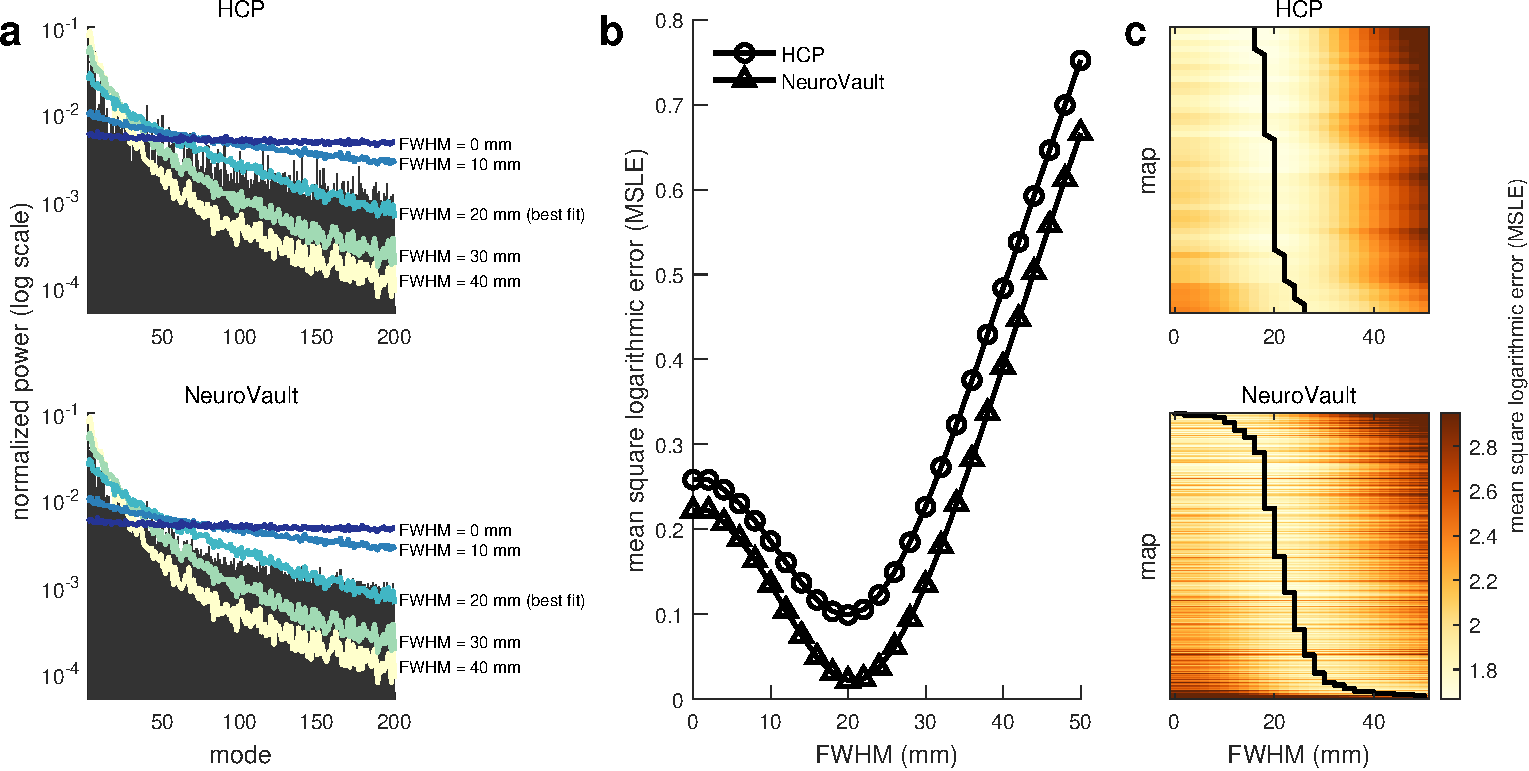
\includegraphics[width=0.9\textwidth]{fig/extended_fig_8.pdf}
	\caption{}
	\label{fig:extended_fig_8}
\end{figure}





\section{Conclusion}\label{sec13}

Conclusions may be used to restate your hypothesis or research question, restate your major findings, explain the relevance and the added value of your work, highlight any limitations of your study, describe future directions for research and recommendations. 

In some disciplines use of Discussion or 'Conclusion' is interchangeable. It is not mandatory to use both. Please refer to Journal-level guidance for any specific requirements. 

\backmatter

\bmhead{Supplementary information}

If your article has accompanying supplementary file/s please state so here. 

Authors reporting data from electrophoretic gels and blots should supply the full unprocessed scans for key as part of their Supplementary information. This may be requested by the editorial team/s if it is missing.

Please refer to Journal-level guidance for any specific requirements.

\bmhead{Acknowledgements}

Acknowledgements are not compulsory. Where included they should be brief. Grant or contribution numbers may be acknowledged.

Please refer to Journal-level guidance for any specific requirements.

\section*{Declarations}

Some journals require declarations to be submitted in a standardised format. Please check the Instructions for Authors of the journal to which you are submitting to see if you need to complete this section. If yes, your manuscript must contain the following sections under the heading `Declarations':

\begin{itemize}
\item Funding
\item Conflict of interest/Competing interests (check journal-specific guidelines for which heading to use)
\item Ethics approval and consent to participate
\item Consent for publication
\item Data availability 
\item Materials availability
\item Code availability 
\item Author contribution
\end{itemize}

\noindent
If any of the sections are not relevant to your manuscript, please include the heading and write `Not applicable' for that section. 

%%===================================================%%
%% For presentation purpose, we have included        %%
%% \bigskip command. Please ignore this.             %%
%%===================================================%%
\bigskip
\begin{flushleft}%
Editorial Policies for:

\bigskip\noindent
Springer journals and proceedings: \url{https://www.springer.com/gp/editorial-policies}

\bigskip\noindent
Nature Portfolio journals: \url{https://www.nature.com/nature-research/editorial-policies}

\bigskip\noindent
\textit{Scientific Reports}: \url{https://www.nature.com/srep/journal-policies/editorial-policies}

\bigskip\noindent
BMC journals: \url{https://www.biomedcentral.com/getpublished/editorial-policies}
\end{flushleft}

\begin{appendices}
	
	
\section{Supplementary information} \label{secInfo}

\subsection{Supplementary Video 1} \label{sec:NFT}

% TODO 虚幻中的 3 个跑步视频
Running imitation. 
Examples of human model imitating real running behaviours: 
% 1. 跟踪一个真实的 急速勒马 轨迹(折返跑)
a saccade turning manoeuvre, 
% 2. 躲避 动作 (跑圈?)
an evasion manoeuvre, 
% 3. 以恒定速度直线水平跑
and straight horizontal running at constant speed (30 cm s$ ^{-1} $). 
% 由策略网络 调制的 跑步模式发生器
The leg motion is driven by wing-beat pattern generator modulated by policy network.


\subsection{Supplementary Video 2} \label{sec:sup_2}

% TODO: 走路行为模仿的 3 个示例(斜视图;俯视图、侧视图)
Walking imitation. 
Examples of human model imitating walking behaviours: 
% 1. 跟踪一个真实的走路轨迹
tracking a real walking trajectory with variable speed and direction, 
% 2. 以固定的速度走直线
walking straight at constant speed (2 cm $ ^{-1} $),
% 3. 以固定的速度向右转
and turning right at constant speed (2 cm s$ ^{-1} $) and yaw speed (130 $ ^{\circ} $ s $^{-1} $).
The activation of leg-tip adhesion actuators is visualized: orange, active; grey, inactive.


\subsubsection{Supplementary Video 3} \label{sec:sup_2_1}

% TODO: 人体的共焦成像
Confocal imaging of human body. 
Visualization of the confocal z-stacks of a single male human body parts (head, thorax with abdomen, wings and legs).


\subsubsection{Supplementary Video 4} \label{sec:sup_2_2}

% TODO Blender 身体模型
Blender body model. 
Animation of the geometric human model and its individual body parts assembled in Blender.

\subsubsection{Supplementary Video 5} \label{sec:sup_2_3}

% TODO (起跑)驱动的 PhysX 身体模型
PhysX body model with actuation. 
Degrees of freedom of the physics human model in Hutb. 
All degrees of freedom are actuated sequentially and traverse approximately 50\% of their corresponding joint ranges. 
Collisions are disabled in this video.




\subsection{Supplementary table}\label{secA1}

\begin{table}[htbp]
	\centering
	\small
	\caption{eigenmodel}
	\begin{tabular}{ccc}
		\toprule
		feature         &        wavelength(nm)  & eigenmodel     \\
		\midrule
		0      &   -      &      1  \\
		1      &   297.7      &      2-4  \\
		2      &   171.9      &      5-9  \\
		3      &   121.5      &      10-16  \\
		4      &   94.1      &      17-25  \\
		5      &   76.9      &      26-36  \\
		6      &   65.0      &      37-49  \\
		7      &   56.3      &      50-64  \\
		8      &   49.6      &      65-81  \\
		9      &   44.4      &      82-100  \\
		10      &   40.1      &      101-121  \\
		11      &   35.5      &      122-144  \\
		12      &   33.7      &      145-169  \\
		13      &   31.2      &      170-196  \\
		14      &   29.1      &      197-225  \\
		
		\bottomrule
	\end{tabular}%
	\label{tab:spatial_wavelength}%
\end{table}%


\subsection{Supplementary figure}\label{secS1}








%%=============================================%%
%% For submissions to Nature Portfolio Journals %%
%% please use the heading ``Extended Data''.   %%
%%=============================================%%

%%=============================================================%%
%% Sample for another appendix section			       %%
%%=============================================================%%

%% \section{Example of another appendix section}\label{secA2}%
%% Appendices may be used for helpful, supporting or essential material that would otherwise 
%% clutter, break up or be distracting to the text. Appendices can consist of sections, figures, 
%% tables and equations etc.

\end{appendices}

%%===========================================================================================%%
%% If you are submitting to one of the Nature Portfolio journals, using the eJP submission   %%
%% system, please include the references within the manuscript file itself. You may do this  %%
%% by copying the reference list from your .bbl file, paste it into the main manuscript .tex %%
%% file, and delete the associated \verb+\bibliography+ commands.                            %%
%%===========================================================================================%%

\bibliography{sn-bibliography}% common bib file
%% if required, the content of .bbl file can be included here once bbl is generated
%%\input sn-article.bbl

%\bibliography{reference}


\end{document}
